\chapter{Hand Features and Representations}

Different hand feature representation and encoding methods are compared. The
hand features can be extracted from either color, depth or both images. 
\begin{figure}[tbh]
  \centering
  \subfigure[Color images] {
	\includegraphics[width=0.45\textwidth]{figures/color_hand.png} 
  }
  \subfigure[Depth images] {
  	\includegraphics[width=0.45\textwidth]{figures/depth_hand.png}
  }
  \caption{$64\times64$ pixel raw image patches of hands.} \label{fig:hand}
\end{figure}

\begin{figure}[tbh]
\centering
\includegraphics{figures/hand3d.png}
\caption{View of quantized depth data of a hand in 3D.}
\end{figure}

During training, all the features are standardized to have 0 mean and 1 standard
deviation using all the training data before being input to the recognition
module. During testing, the data are standardized using the mean and and
standard deviation from training.

\section{Motion Features}
We use both the Kinect and the Xsens data from the ChAirGest corpus~\cite{Ruffieux2013} to
extract hand motion feature vectors for gesture modeling.

It is relatively easy to obtain features from the Xsens data. We choose to use linear
acceleration (x, y, z), angular velocity (x, y, z) and Euler orientation (yaw, pitch, roll)
from the Xsens unit on the hand to form a 9-dimensional feature vector $\underline{x}_t^{\text{xsens}}$
for every time frame $t$.

From hand tracking using a Kinect sensor, we can extract the position of the
gesturing hand in $(x, y, z)$ coordinates relative to the shoulder center joint to
form a 3-dimensional vector. From this, we can again compute  the 
velocity and and acceleration, all in 3D world coordinates. The feature vector
is computed for each input frame streamed from the sensor to form a sequence of
feature vectors.

Combining the two, we
have a 12-dimensional feature vector $\underline{x}_t = [\underline{x}^\text{kinect}_t, \underline{x}^\text{xsens}_t]$.

It is also useful to apply temporal smoothing on the motion data. In our
real-time system, we apply ``box'' smoothing (i.e., simple and linear smoothing
with equal weight) with a window size of 15 frames on the relative positions of
the gesturing hand.

Figure~\ref{fig:motion-hist-rest} shows the histograms of the standardized $(x,
y, z)$ coordinates of relative position, velocity and acceleration from one user's
data in the YANG dataset. The peak values corresponds to rest positions.
Figure~\ref{fig:motion-hist} shows the histogram of the same data excluding
those from rest position. We can see that the distribution roughly follows
Gaussian or mixture of Gaussians distributions.

\begin{figure}[tbh]
\centering
\subfigure[]{
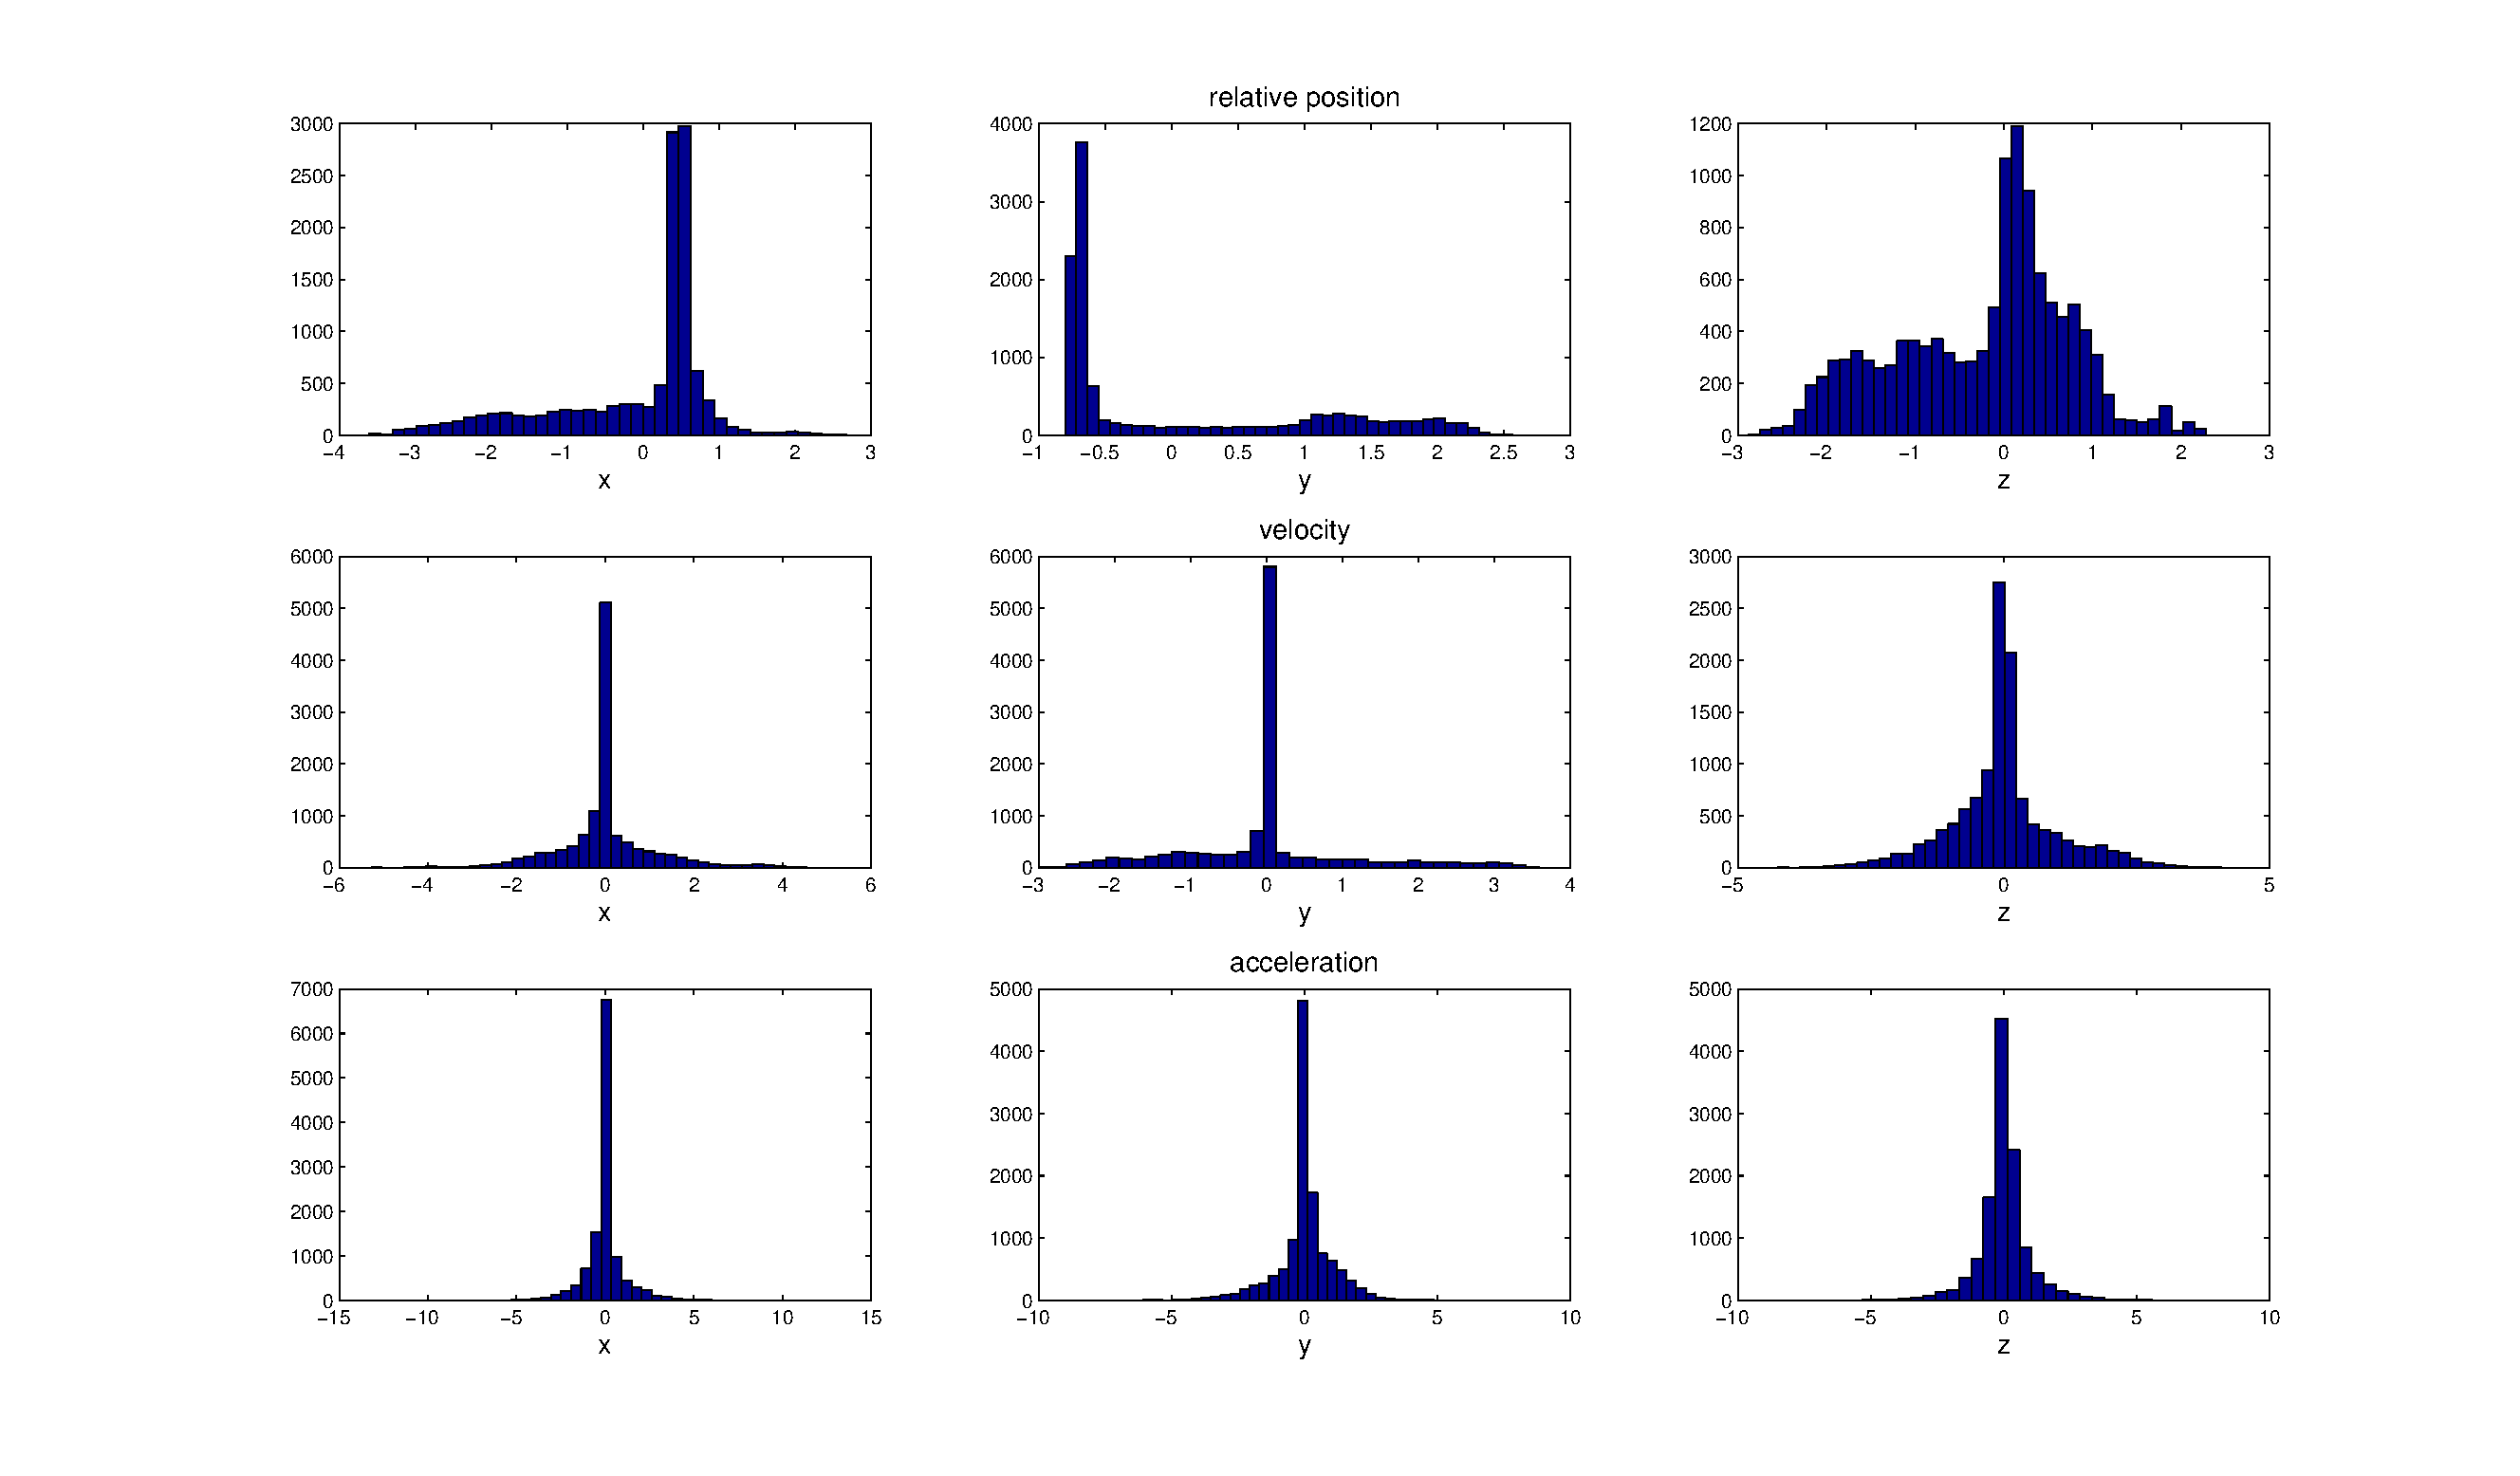
\includegraphics[trim=30mm 15mm 30mm 10mm,
clip, width=\columnwidth]{figures/motion_hist_rest.eps}
\label{fig:motion-hist-rest}
}
\subfigure[]{
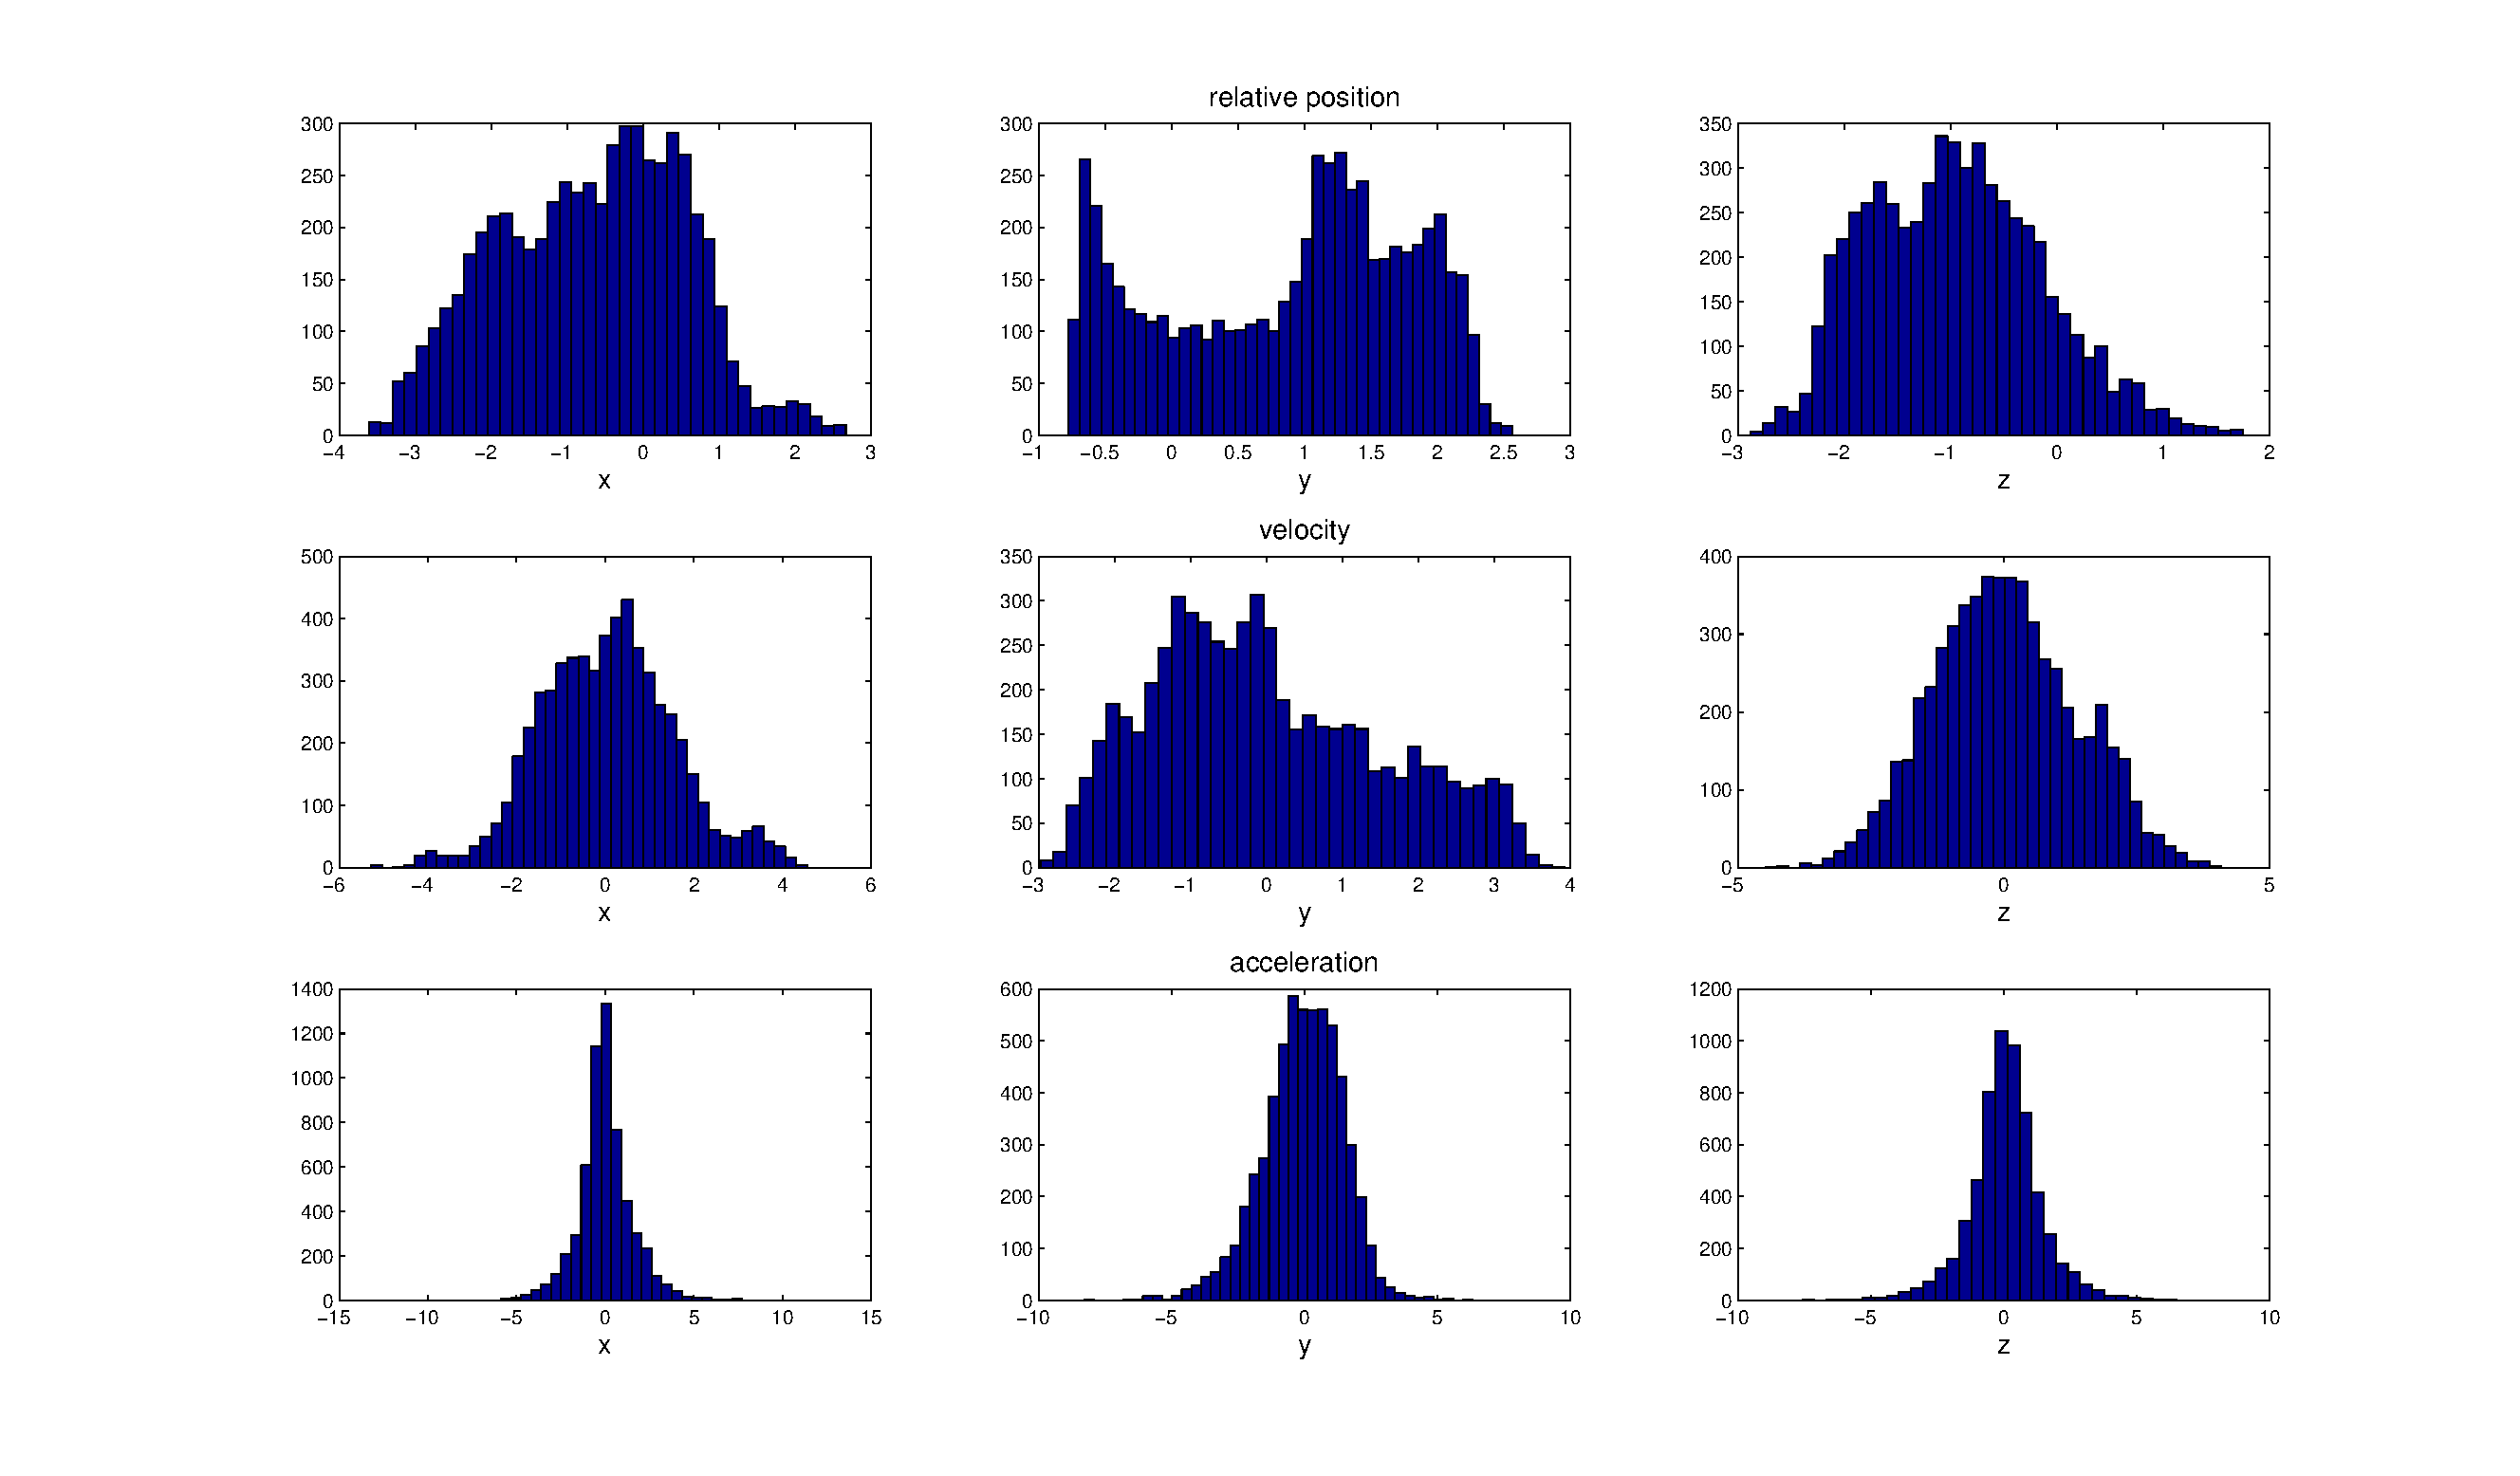
\includegraphics[trim=30mm 15mm 30mm 10mm,
clip, width=\columnwidth]{figures/motion_hist.eps}
\label{fig:motion-hist}
}
\caption{Histograms of motion features.}
\end{figure}

Try Xsens data on hand, quarternion.

\section{Histogram of Oriented Gradients}
For each pixel, the magnitude of gradient is 
\begin{align*}
m = \sqrt{dx^2 + dy^2}
\end{align*}

If an image $I$ has dimensions $m\times n$, the size of the computed feature
vector $H$ is $(m/\text{cell\_size} - fold_per_dim) \times (n/\text{cell\_size}
- fold_per_dim) \times \text{num\_bin}$.

\begin{figure}[tbh]
  \centering
  \subfigure[Color] {
  \includegraphics[width=0.45\textwidth]{figures/color_denoised_5.png} 
  }
  \subfigure[Depth] {
    \includegraphics[width=0.45\textwidth]{figures/depth_denoised_5.png}
  }
  \subfigure[Color HOG] {
  \includegraphics[width=0.45\textwidth]{figures/color_hog.png} }
  \subfigure[Depth HOG] {
    \includegraphics[trim={0cm 1.5cm 0cm 0cm},
  clip, width=0.5\textwidth]{figures/depth_hog.png}
  }
  \caption{$64\times64$ pixel image patches of hands.} \label{fig:hand}
\end{figure}

\section{SVM for hand pose classification}
We use grid search~\cite{hsu10} on the training data to find the penalty
parameter of the error term, $C$, and $\gamma$ in the radial basis function (RBF) kernel function. 
The search uses 5-fold cross validation and the best parameters found are $C =
0.03$ and $\gamma = 0.03$ with an average accuracy of 95.5\%.

SVM for unbalanced data. \cite{ben2010}
If we ignore the  fact that the data is unbalanced, the resultant classifier
will favor the majority class, in this case the ``other'' category. To take this
into account, we can assign different misclassification (SVM soft-margin
constants) to each class. If $n_1$ and $n_2$ are the number of examples in two
classes, 

\begin{align}
\frac{C_+}{C_-} = \frac{n_-}{n_+}
\end{align}

\begin{figure}[tbh]
\centering
\subfigure[]{
  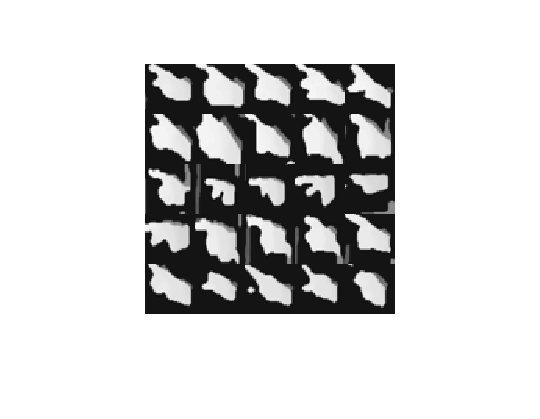
\includegraphics[width=0.5\linewidth,
  trim={0cm 1cm 0cm 0cm}, clip]{figures/point_depth_resize_32_denoise.eps} }
\subfigure[]{
  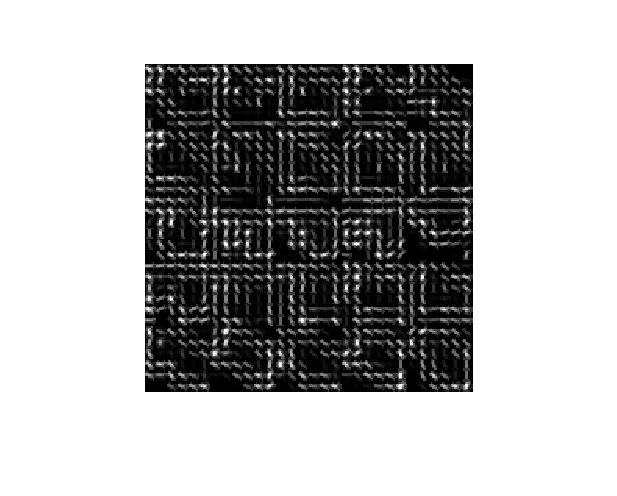
\includegraphics[trim={0cm 1cm 0cm 0cm},
  clip, width=0.45\linewidth]{figures/point_depth_hog.eps} }
\subfigure[]{
  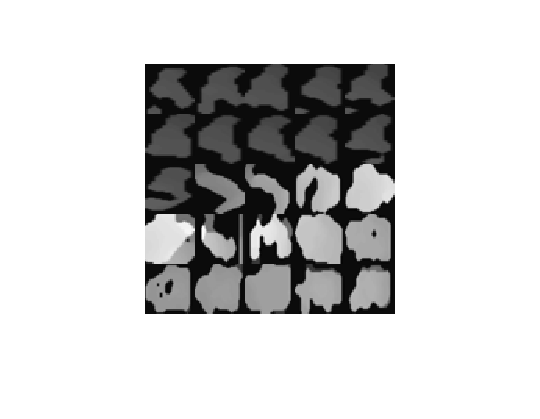
\includegraphics[width=0.5\linewidth,
  trim={0cm 1cm 0cm 0cm}, clip]{figures/other_depth_resize_32_denoise.eps} }
\subfigure[]{
  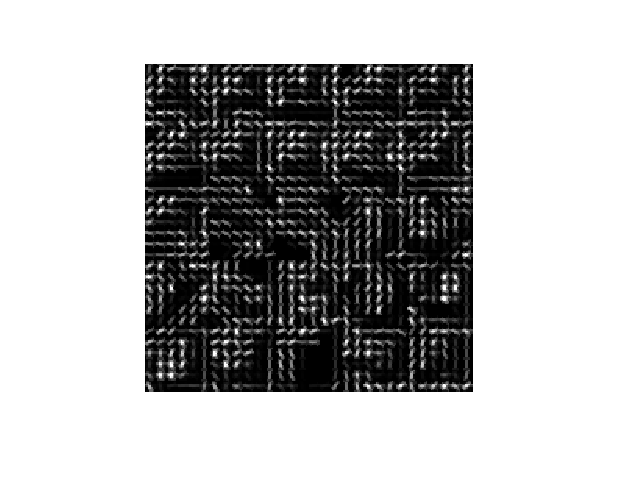
\includegraphics[trim={0cm 1cm 0cm 0cm},
  clip, width=0.45\linewidth]{figures/other_depth_hog.eps} }
\end{figure}

Radial Basis Function (RBF) kernel, use grid search to find best parameters, C =
0.03, $\gamma = 0.5$. Ratio between point pose and other poses is 27 : 73, so
the weight for $C_other$ and $C_point$ is 73 : 27. 

no standardization.

Test accuracy 92.6282\% (289/312) 2-class classfication

The probabilities from SVM is not Gaussian. 

\begin{figure}[tbh]
\centering
\includegraphics{figures/hist_svm.eps}
\caption{}
\label{}
\end{figure}

One user data, hand pose gestures, 5 classes
results on hand pose gestures
precision: 0.74, recall: 0.77, F1: 0.75

Compare with Gaussian
precision: 0.81, recall: 0.82, F1: 0.81

\begin{figure}[tbh]
\centering
\includegraphics{figures/svm_hmm.png}
\end{figure}

\section{Dictionary Learning}

\section{Principal Component Analysis}
We use Principal Component Analysis (PCA)~\cite{pca} to reduce the
dimensionality of the HOG features. The number of principal components to use
is determined through cross-validation. For the YANG dataset, we use 15
principal components from the HOG features. We use one
user's data from the YANG dataset to visualize the PCA
encoded HOG features. Figure~\ref{fig:pca} shows the histograms of the 15
variables after projecting the original HOG feature data onto the principal
components and then being standardized.
We observe that the distributions closely follow Gaussian or mixture of
Gaussians distributions.

\begin{figure}[tbh]
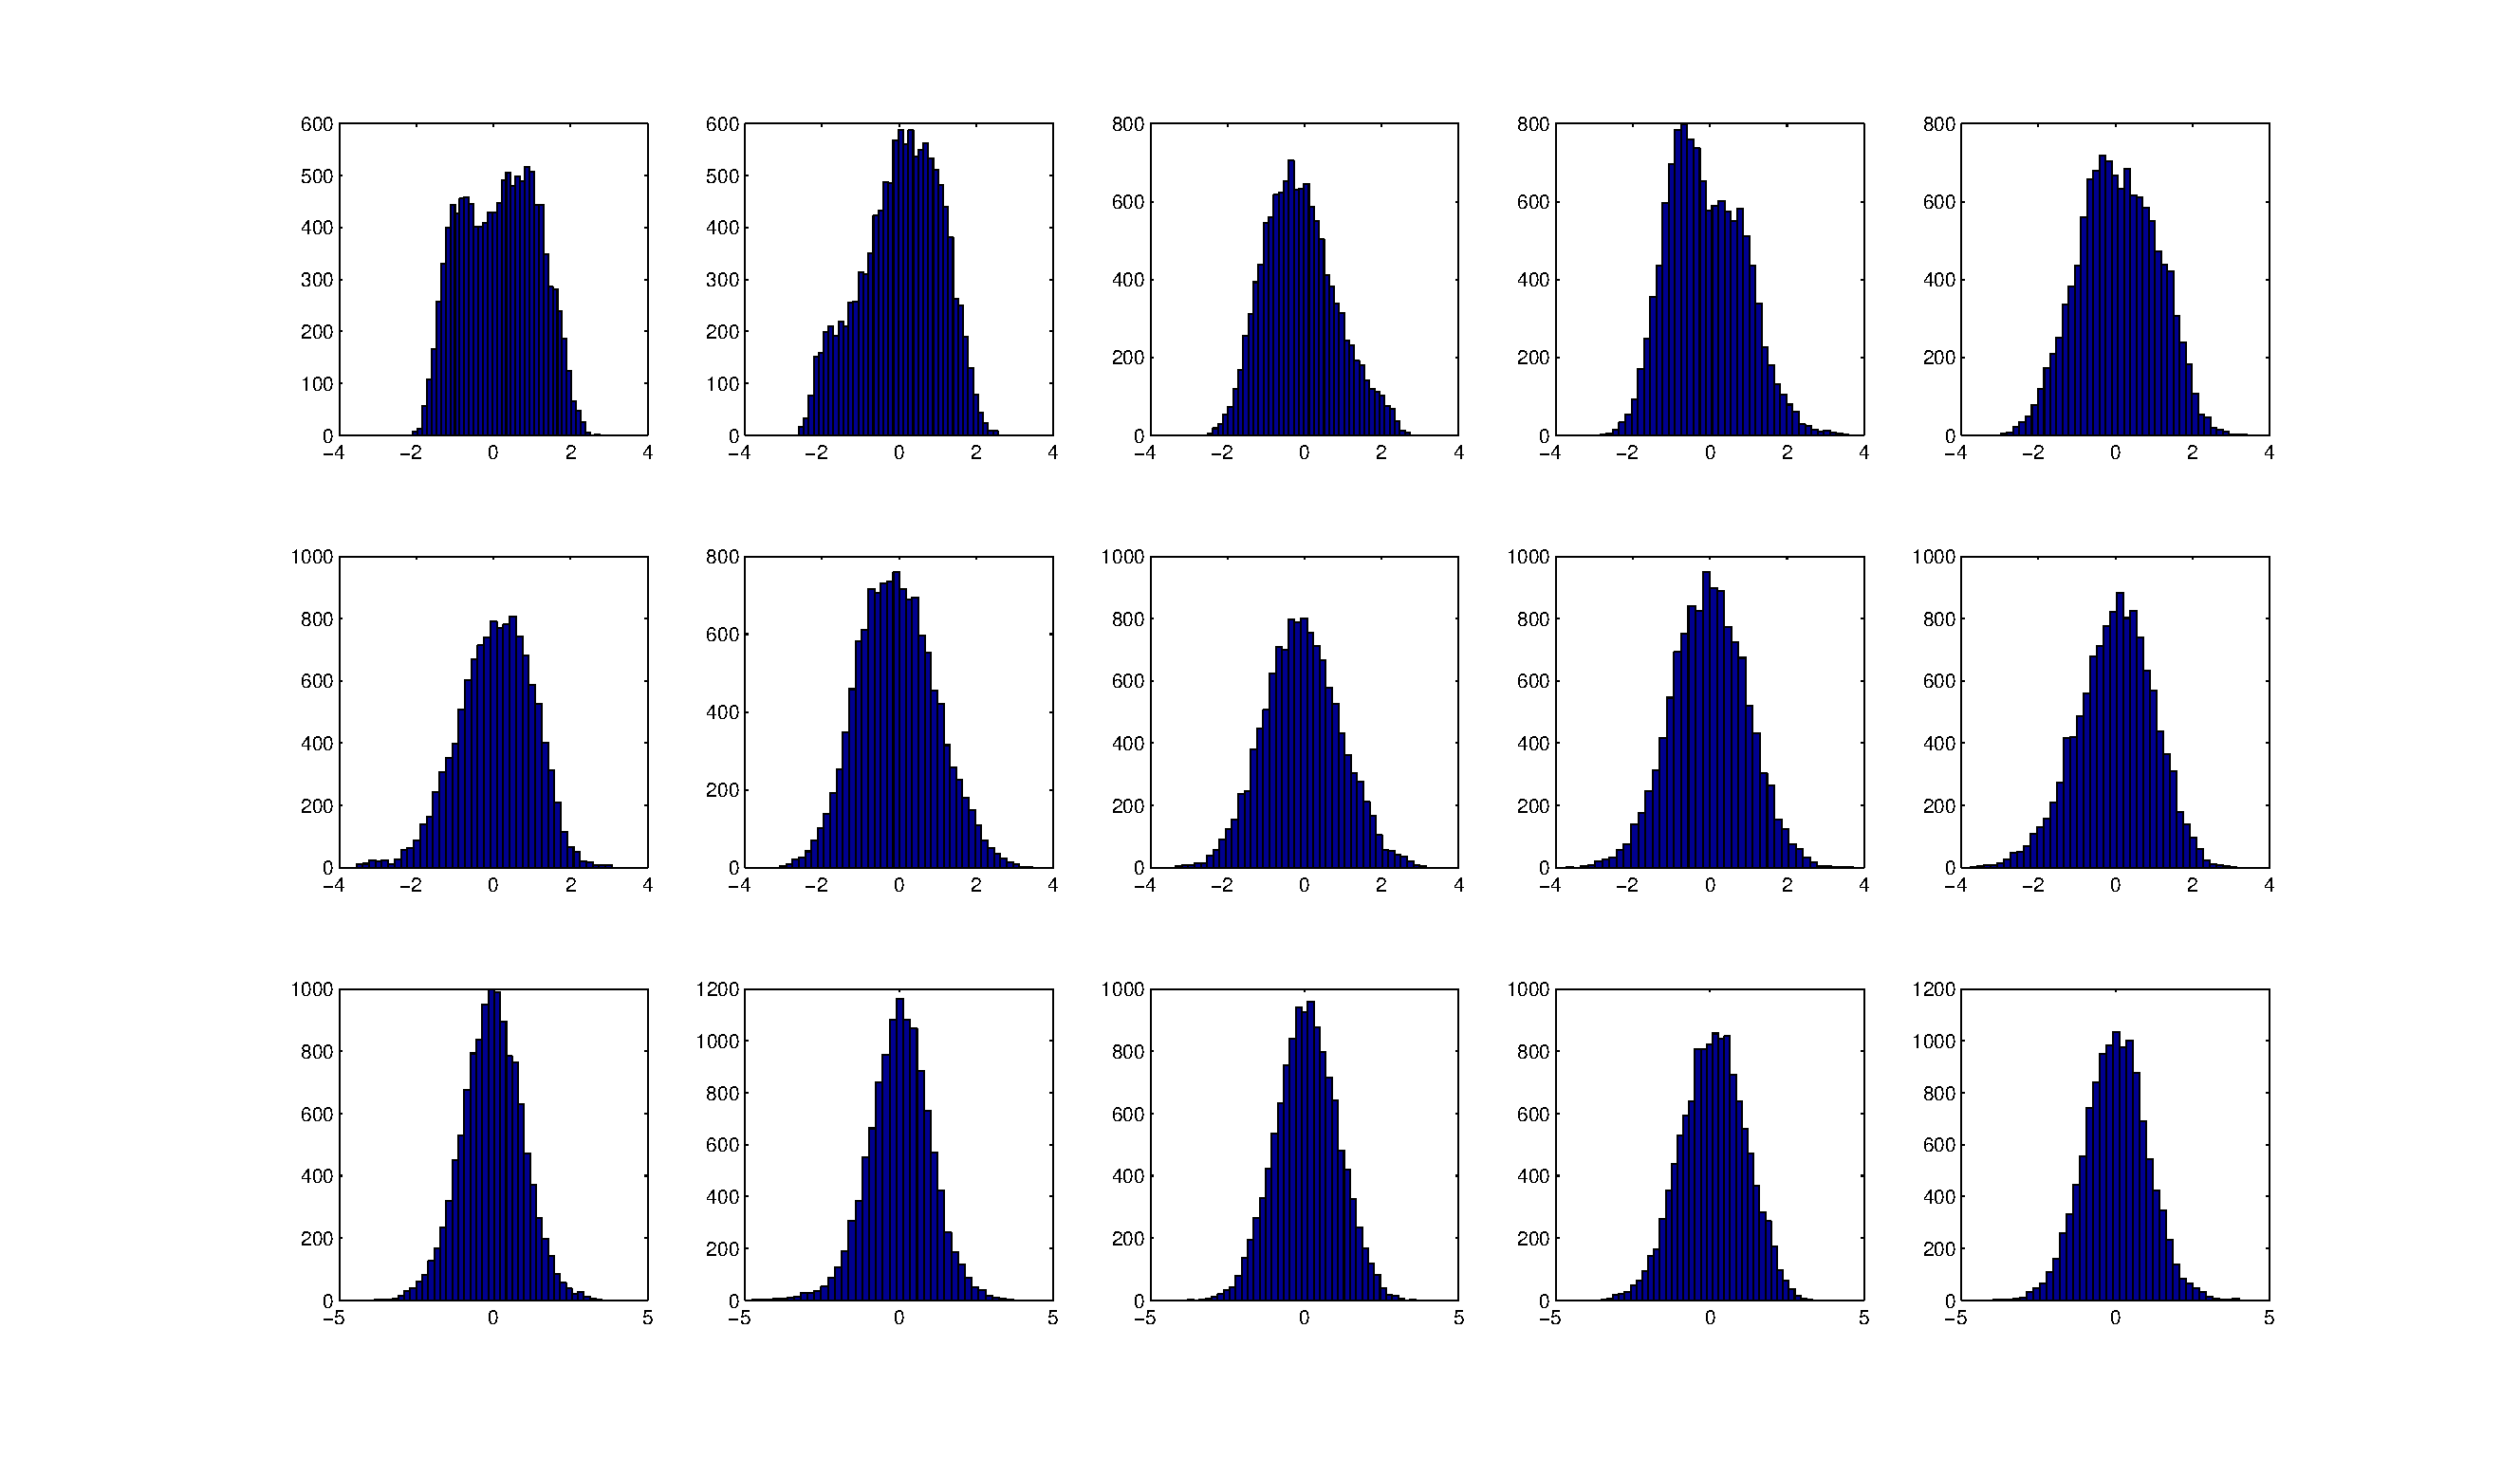
\includegraphics[width=\columnwidth]{figures/hist_pca.eps}
\caption{}
\label{fig:pca}
\end{figure}

\section{Discussion}